\documentclass[13pt,a4paper]{article}
\usepackage[spanish,es-nodecimaldot]{babel}	% Utilizar español
\usepackage[utf8]{inputenc}					% Caracteres UTF-8
\usepackage{graphicx}						% Imagenes
\usepackage[hidelinks]{hyperref}			% Poner enlaces sin marcarlos en rojo
\usepackage{fancyhdr}						% Modificar encabezados y pies de pagina
\usepackage{float}							% Insertar figuras
\usepackage[textwidth=390pt]{geometry}		% Anchura de la pagina
\usepackage[nottoc]{tocbibind}				% Referencias (no incluir num pagina indice en Indice)
\usepackage{enumitem}						% Permitir enumerate con distintos simbolos
\usepackage[T1]{fontenc}					% Usar textsc en sections
\usepackage{amsmath}						% Símbolos matemáticos
\usepackage[ruled,vlined]{algorithm2e}      % Pseudocódigo
\usepackage{xcolor}
\usepackage{listings}
% Para que acepten tíldes los listing
\lstset{     
     literate=%
         {á}{{\'a}}1
         {é}{{\'e}}1
         {í}{{\'i}}1
         {ó}{{\'o}}1
         {ú}{{\'u}}1
         {Á}{{\'A}}1
         {É}{{\'E}}1
         {Í}{{\'I}}1
         {Ó}{{\'O}}1 
         {Ú}{{\'U}}1
         {ñ}{{\~n}}1 
         {Ñ}{{\~N}}1 
         {¿}{{?``}}1 
         {¡}{{!``}}1
}
\usepackage{dsfont}
\usepackage{subfigure}

% ==============================================================================

\usepackage{caption}
\usepackage[section]{placeins}
\makeatletter
\def\fps@figure{H}
\makeatother

\usepackage{booktabs}
\usepackage{longtable}
\usepackage{array}
\usepackage{multirow}
\usepackage{wrapfig}
\usepackage{colortbl}
\usepackage{pdflscape}
\usepackage{tabu}
\usepackage{threeparttable}
\usepackage{threeparttablex}
\usepackage[normalem]{ulem}
\usepackage{makecell}
\usepackage{xcolor}
\usepackage[bottom]{footmisc}

% ==============================================================================
% ==============================================================================

% Comando para poner el nombre de la asignatura
\newcommand{\asignatura}{Big Data I}
\newcommand{\autor}{Ignacio Vellido Expósito}
\newcommand{\titulo}{Cloud Computing y Big Data}
\newcommand{\subtitulo}{Práctica sobre Contenedores}

% Configuracion de encabezados y pies de pagina
\pagestyle{fancy}
\lhead{\autor{}}
\rhead{\asignatura{}}
\lfoot{Máster Ciencia de Datos e Ingeniería de Computadores}
\cfoot{}
\rfoot{\thepage}
\renewcommand{\headrulewidth}{0.4pt}		% Linea cabeza de pagina
\renewcommand{\footrulewidth}{0.4pt}		% Linea pie de pagina

% ==============================================================================
% ==============================================================================

\begin{document}
    \pagenumbering{gobble}
    % ==============================================================================
% Pagina de titulo
\begin{titlepage}
    \begin{minipage}{\textwidth}
        \centering

        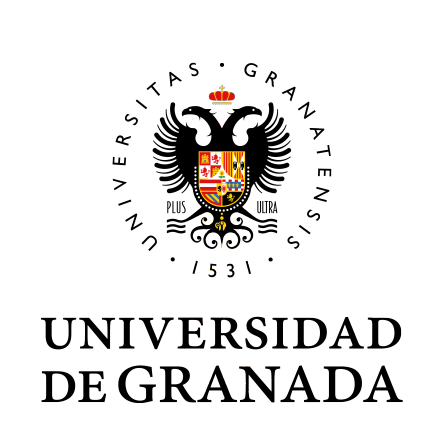
\includegraphics[scale=0.5]{img/ugr.png}\\

        \textsc{\Large \asignatura{}\\[0.2cm]}
        \textsc{MÁSTER CIENCIA DE DATOS E INGENIERÍA DE COMPUTADORES}\\[1cm]

        \noindent\rule[-1ex]{\textwidth}{1pt}\\[1.5ex]
        \textsc{{\Huge \titulo\\[0.5ex]}}
        \textsc{{\Large \subtitulo\\}}
        \noindent\rule[-1ex]{\textwidth}{2pt}\\[2.5ex]

        \end{minipage}

        \vspace{0.3cm}

        \begin{minipage}{\textwidth}

        \centering

        \textbf{Autor}\\ {\autor{} \\ ignaciove@correo.ugr.es}\\[1.5ex]
        \vspace{0.4cm}

        
\includegraphics[scale=0.3]{img/etsiit.jpeg}
        
\includegraphics[scale=0.6]{img/master.png}

        \vspace{0.7cm}
        \textsc{Escuela Técnica Superior de Ingenierías Informática y de Telecomunicación}\\
        \vspace{1cm}
        \textsc{Curso 2020-2021}
    \end{minipage}
\end{titlepage}
% ==============================================================================
    
    \pagenumbering{arabic}
    \tableofcontents
    \thispagestyle{empty}				% No usar estilo en la pagina de indice

    \newpage

    % ==============================================================================

    \section{Contenedor con SGDB MySQL}

\subsection{Descripción}

Contendor docker partiendo de una instalación base de MariaDB

\subsection{Archivo Dockerfile}

\subsection{Proceso de construcción}

\subsubsection{En hadoop.ugr.es}

\subsubsection{En Azure}

\subsection{Evaluación}

Para la evaluación del contenedor se añade una pequeña base de datos sobre la que se realizan las siguientes pruebas.

% Acceso desde local
% Acceso desde remoto \newpage
    \section{Contenedor para actividades de ciencia de datos basado en Python}

\subsection{Descripción}

Contenedor partiendo de una imagen base de Ubuntu al que se le añade Python con distintos paquetes de ciencia de datos, concretamente:
\begin{itemize}
    \item pandas, numpy, scikit-learn
    % \item scikit-learn
    \item seaborn, scipy
    % \item scipy
    % \item numpy
    \item matplotlib, xlrd
    % \item xlrd
\end{itemize}

\subsection{Archivo Dockerfile}

Para la construcción del archivo Dockerfile se parte de las recomendaciones de \url{https://hub.docker.com/_/python} y se adapta para una instalación base de Ubuntu.

\begin{figure}[H]\center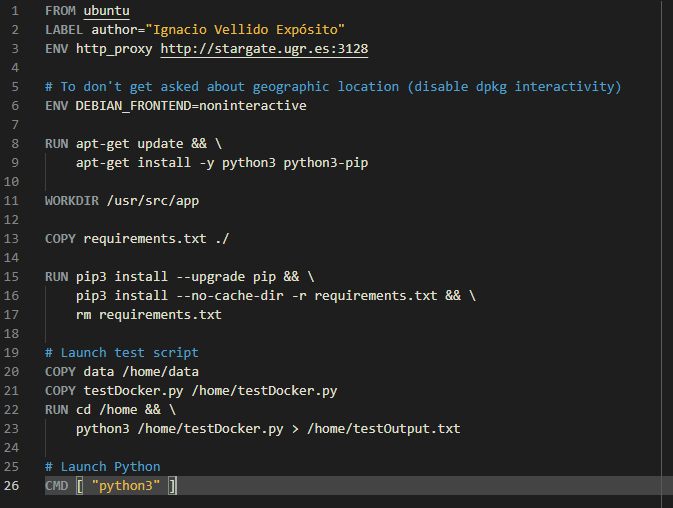
\includegraphics[width=.82\linewidth]{img/python/p0.png}\caption{}\end{figure}

\begin{figure}[H]\center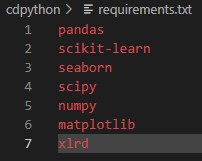
\includegraphics[width=.25\linewidth]{img/python/p0-2.png}\caption{Archivo con los paquetes a instalar.}\end{figure}

\subsection{Proceso de construcción}

\subsubsection{En hadoop.ugr.es}

\begin{figure}[H]\center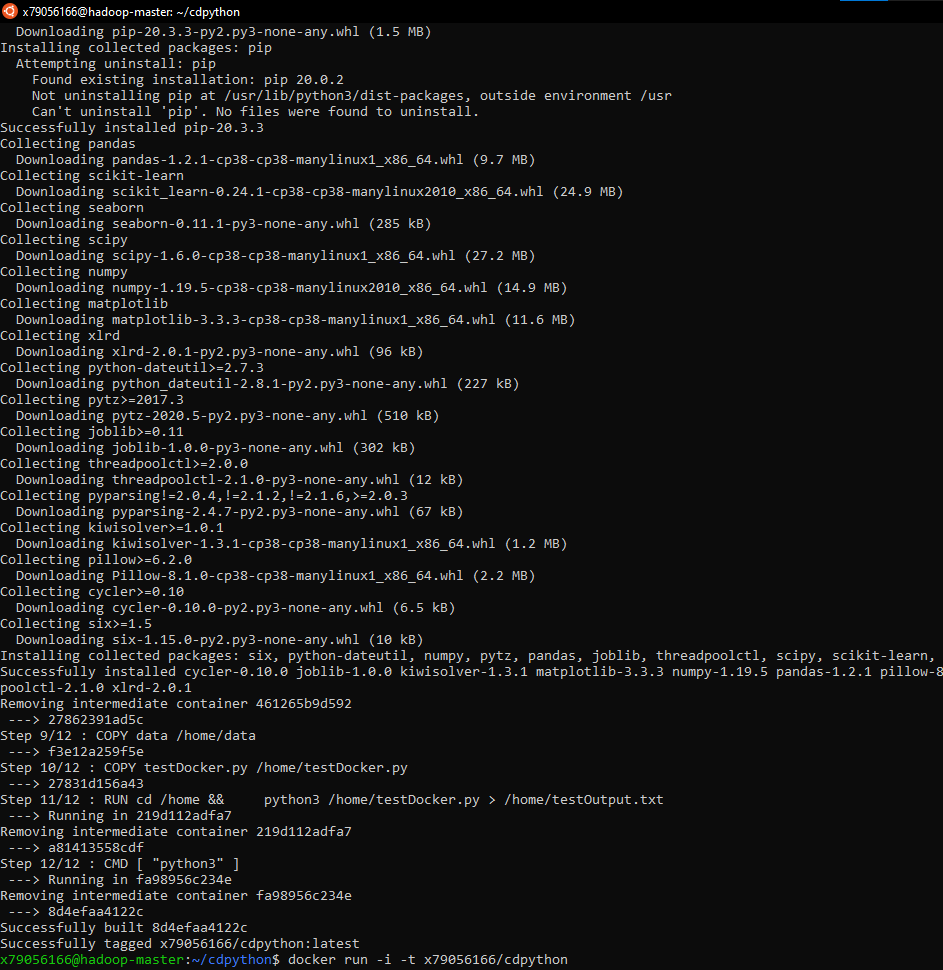
\includegraphics[width=.95\linewidth]{img/python/p1.png}\caption{Construcción de la imagen.}\end{figure}

\begin{figure}[H]\center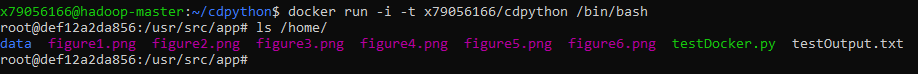
\includegraphics[width=.95\linewidth]{img/python/p2.png}\caption{Lanzando la imagen.}\end{figure}

\begin{figure}[H]\center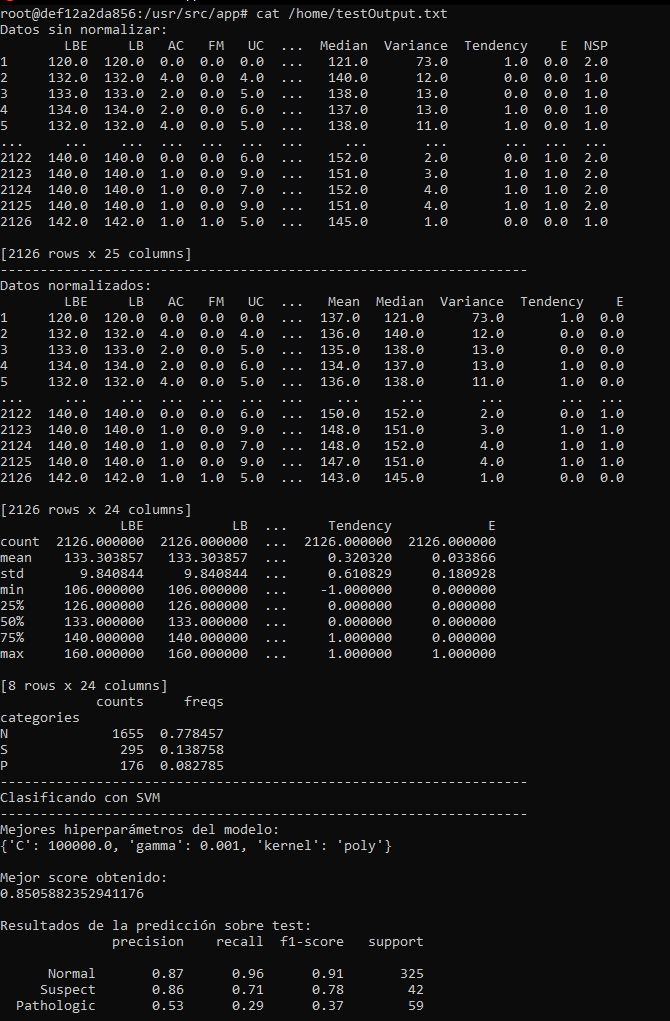
\includegraphics[width=.95\linewidth]{img/python/p3.png}\caption{Contenido de la imagen.}\end{figure}

\begin{figure}[H]\center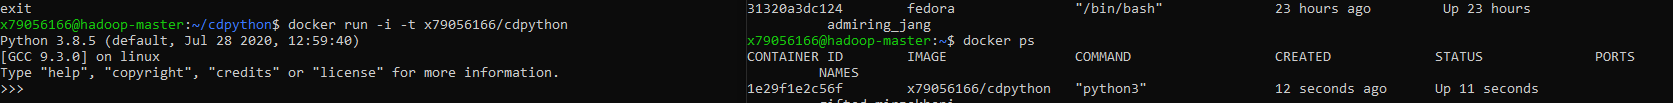
\includegraphics[width=.99\linewidth]{img/python/p5.png}\caption{Comprobando ejecución.}\end{figure}

\subsubsection{En Azure}

Los pasos para desplegar la imagen en Azure son los mismos que con el contenedor de R. Es necesario modificar el Dockerfile y subirlo al repositorio, e indicarle a Azure dónde encontrar la imagen.

\begin{figure}[H]\center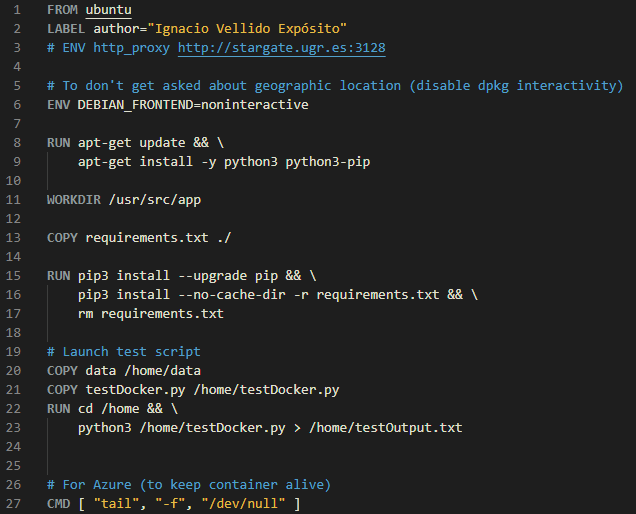
\includegraphics[width=.95\linewidth]{img/python/p10.png}\caption{Dockerfile desplegado en Azure.}\end{figure}

\begin{figure}[H]\center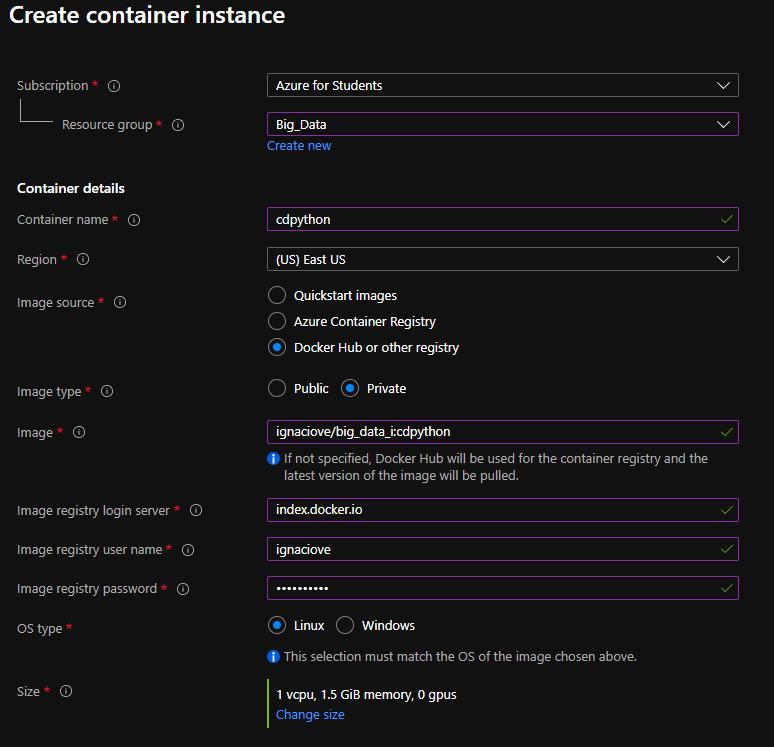
\includegraphics[width=.85\linewidth]{img/python/p7.png}\caption{Despliegue del contenedor en Azure.}\end{figure}

% \begin{figure}[H]\center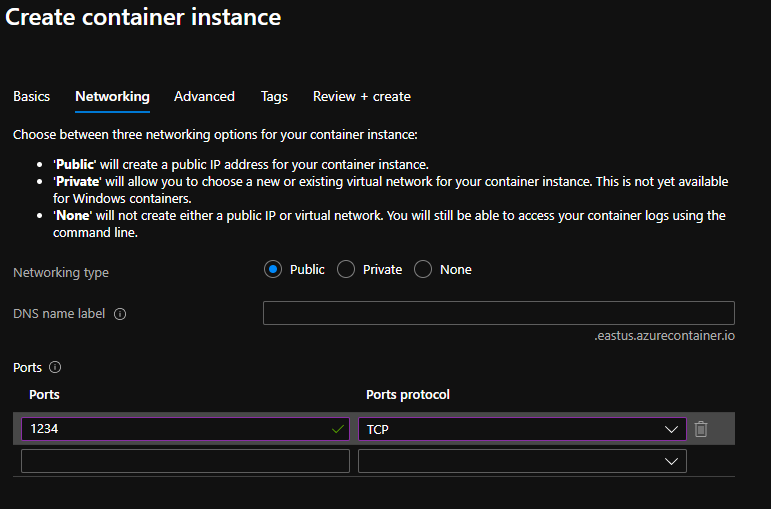
\includegraphics[width=.95\linewidth]{img/python/p8.png}\caption{Indicando puerto a abrir}\end{figure}

\begin{figure}[H]\center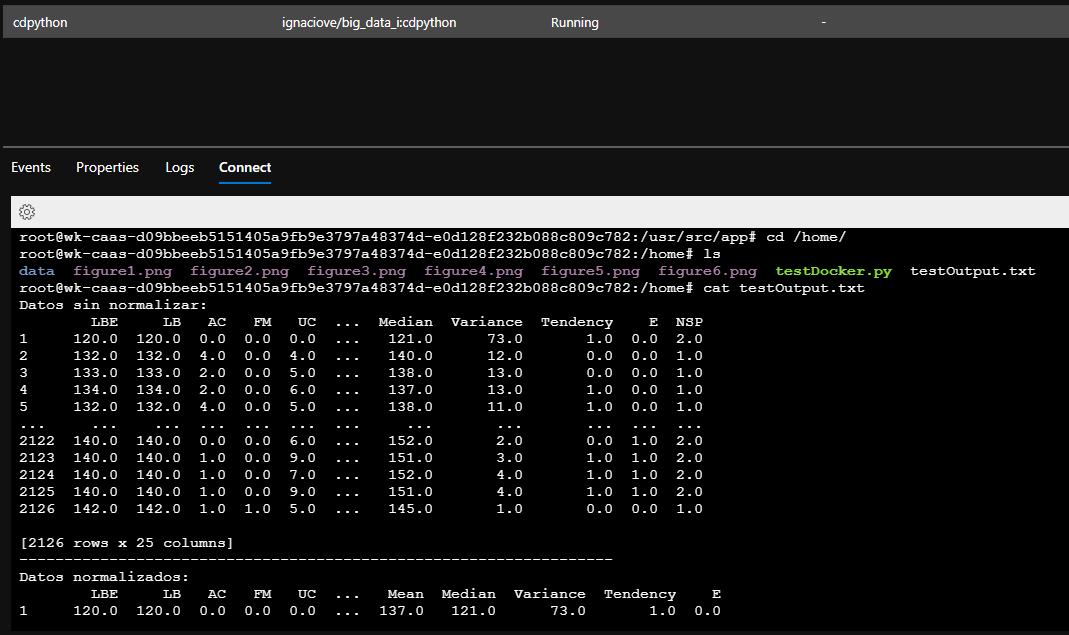
\includegraphics[width=.87\linewidth]{img/python/p9.png}\caption{Imagen del contenedor en ejecución.}\end{figure}

\subsection{Evaluación}

Para evaluar el correcto funcionamiento se lanza el siguiente script, que carga los paquetes instalados y realiza un aprendizaje sobre un conjunto de datos con SVM.

\begin{figure}[H]\center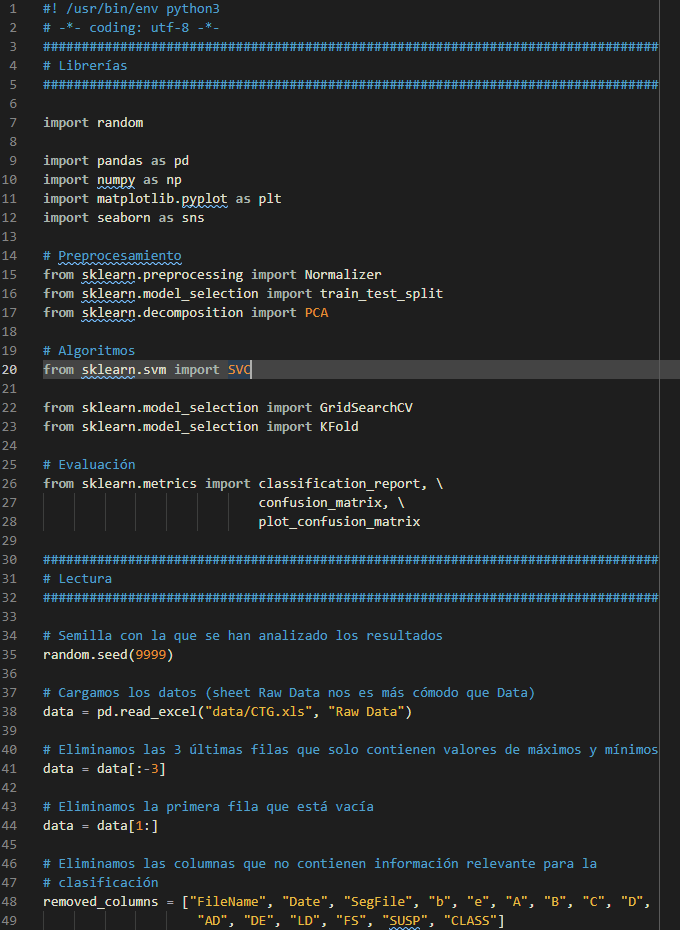
\includegraphics[width=.95\linewidth]{img/python/p6.png}\caption{Parte del script de prueba.}\end{figure} \newpage
    \section{Contenedor para actividades de ciencia de datos basado en R}

\subsection{Descripción}

Contenedor docker partiendo de una instalación base de R al que se le añaden distintos paquetes de ciencia de datos.

\subsection{Archivo Dockerfile}


% MEJOR CAPTURA

% \begin{lstlisting}
% FROM rocker/r-base
% LABEL author="Ignacio Vellido Expósito"
% ENV http_proxy http://stargate.ugr.es:3128

% RUN apt-get update

% # Se podrían separar para evitar que si uno falla se corte
% # la ejecución. Como está testeado se deja resumido
% RUN R -e "install.packages(c('tidyverse','caret','RSNNS',
%                              'frbs','FSinR','forecast'),
%                             dependencies=TRUE, 
%                             repos='http://cran.rstudio.com/')"

% # Para automatizar el proceso de testeo, se lanza desde aquí
% COPY testDocker.R /home/testDocker.R

% # Lanzar script
% CMD R -e "source('/home/testDocker.R')"
% # CMD "R /home/testDocker.R > /home/testOutput.txt"
% \end{lstlisting}

\subsection{Proceso de construcción}

% Captura docker construído

% Captura docker en funcionamiento

% Captura desde dentro del docker

\subsection{Evaluación}

Para evaluar el correcto funcionamiento se lanza el siguiente script, que carga las librerías instaladas y realiza operaciones con algunas de ellas \newpage

    \setlength{\parskip}{1em}
    
    % ==============================================================================
    
    \newpage
    \nocite{*}
    \bibliography{bibliografia}
	\bibliographystyle{plain}
\end{document}

% ==============================================================================
% ==============================================================================